\documentclass[index]{subfiles}
\begin{document}
\chapter{算例:\SI{7.7}{\kilo\watt}车载无线充电系统}\label{sec:example}
为了证明该自动化设计系统强大的分析设计能力,本文对一车载无线充电系统的磁谐振部件进行基本(但并不平凡)的优化设计。

\section{需求分析}\label{sec:example-req}
设传输距离(线圈到线圈)为\SI{200}{\milli\metre},发射端和接收端完全对称,且只考虑平面式单层正方形线圈一种线圈形式。
该系统的谐振频率固定为\SI{85}{\kilo\hertz}。
其线圈采用利兹线绕成,线径\SI{5}{\milli\metre}。
线圈下方\SI{1.5}{\milli\metre}处设正方形PC95铁氧体磁屏蔽层。

现需要同时优化线圈边长、线圈匝数、匝间距、磁屏蔽层厚度、磁屏蔽层边长共计5个参数,使得系统性能同时满足以下几个标准:
\begin{itemize}
  \item 整个系统的尺寸不应超过\SI{500}{\milli\metre}$\times$\SI{500}{\milli\metre},越小越好
  \item 整个接收端(发射端)的厚度\SI{\lte 30}{\milli\metre},越小越好
  \item 正常工况下,线圈互感\SI{=24}{\micro\henry}(可以有\SI{\pm 10}{\percent}的误差),越准越好
  \item 横向偏移\SI{200}{\milli\metre}的情况下,互感\SI{\geq 10}{\micro\henry},越大越好
  \item 线圈电阻\SI{\leq 0.4}{\ohm},越小越好
\end{itemize}

\section{仿真文件准备}
\begin{figure}[h]
  \centering%
  \subcaptionbox{项目结构和磁模型结构\label{fig:example-proj}}
    {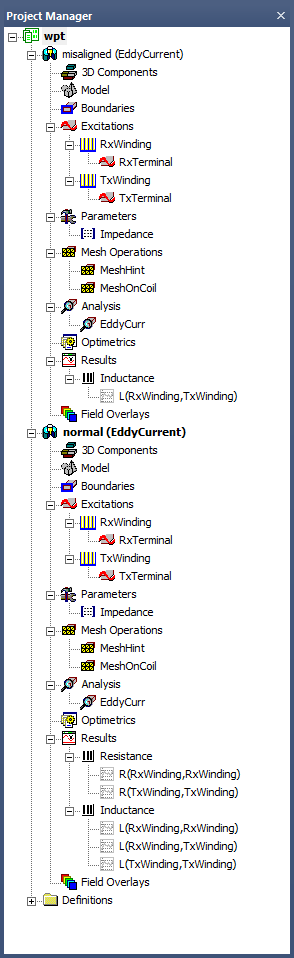
\includegraphics{./figures/example-proj.png}}
  \hspace{1em}
  \subcaptionbox{几何模型结构\label{fig:example-model}}
    {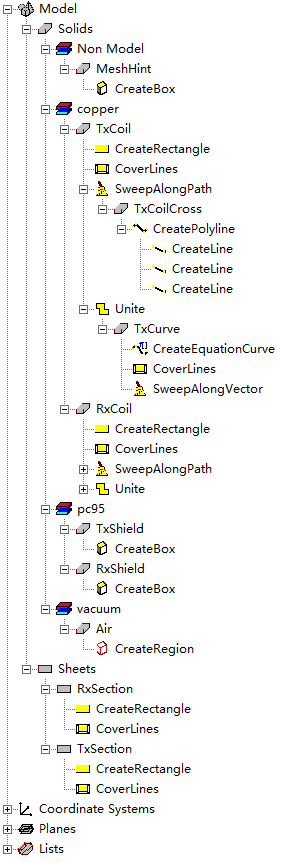
\includegraphics{./figures/example-model.png}}
  \caption[仿真文件的结构]{使用Ansys Maxwell 3D对电动汽车无线充电系统磁谐振部件进行建模。}
\end{figure}

\subsection{项目结构}
从\cref{sec:example-req}中不难看出,对每一种可能设计变量组合,都需要进行两次有限元分析:一次针对正常工况,一次针对横向偏移时。
为此,本文在同一个Ansys项目(Project)中添加normal和misaligned两个设计(Design),以分别对两种情况进行建模,如\cref{fig:example-proj}所示。

为了与自动化设计系统配合,本文设置项目的项目变量(Project Variables)如下:
\begin{description}
  \item[\$tTurns, \$rTurns] 发射/接收线圈匝数,待定
  \item[\$tWidth, \$rWidth] 发射/接收线圈最内圈宽度的一半,待定
  \item[\$tLength, \$rLength] 发射/接收线圈最内圈长度的一半,待定
  \item[\$tInterval, \$rInterval] 发射/接收线圈匝间距,待定
  \item[\$tIns, \$rIns] 发射/接收端绝缘材料的厚度,为\SI{6.5}{\milli\metre}
  \item[\$tExtra, \$rExtra] 发射/接收端磁屏蔽层比线圈最外圈多出来的长度,待定
  \item[\$tShield, \$rShield] 发射/接收端磁屏蔽层的厚度,待定
  \item[\$gap] 传输距离,为\SI{200}{\milli\metre}
  \item[\$crossHeight] 线圈螺旋结构首末链接线的高度,为\SI{2.5}{\milli\metre}
  \item[\$lineSize] 线圈截面正方形的边长的一半,为$2.5\times\frac{\sqrt{\pi}}{2}=\SI{2.2155673136319}{\milli\metre}$
\end{description}

对于设计misaligned,设置设计变量(Design Variables)如下:
\begin{description}
  \item[\$xMis] 沿X轴的横向偏移,为\SI{200}{\milli\metre}
  \item[\$yMis] 沿Y轴的横向偏移,为\SI{0}{\milli\metre}
\end{description}

\subsection{搭建几何模型}
\begin{figure}[h]
  \centering%
  \subcaptionbox{建模过程中用到的正方形线圈的轮廓\label{fig:example-curve}}
    {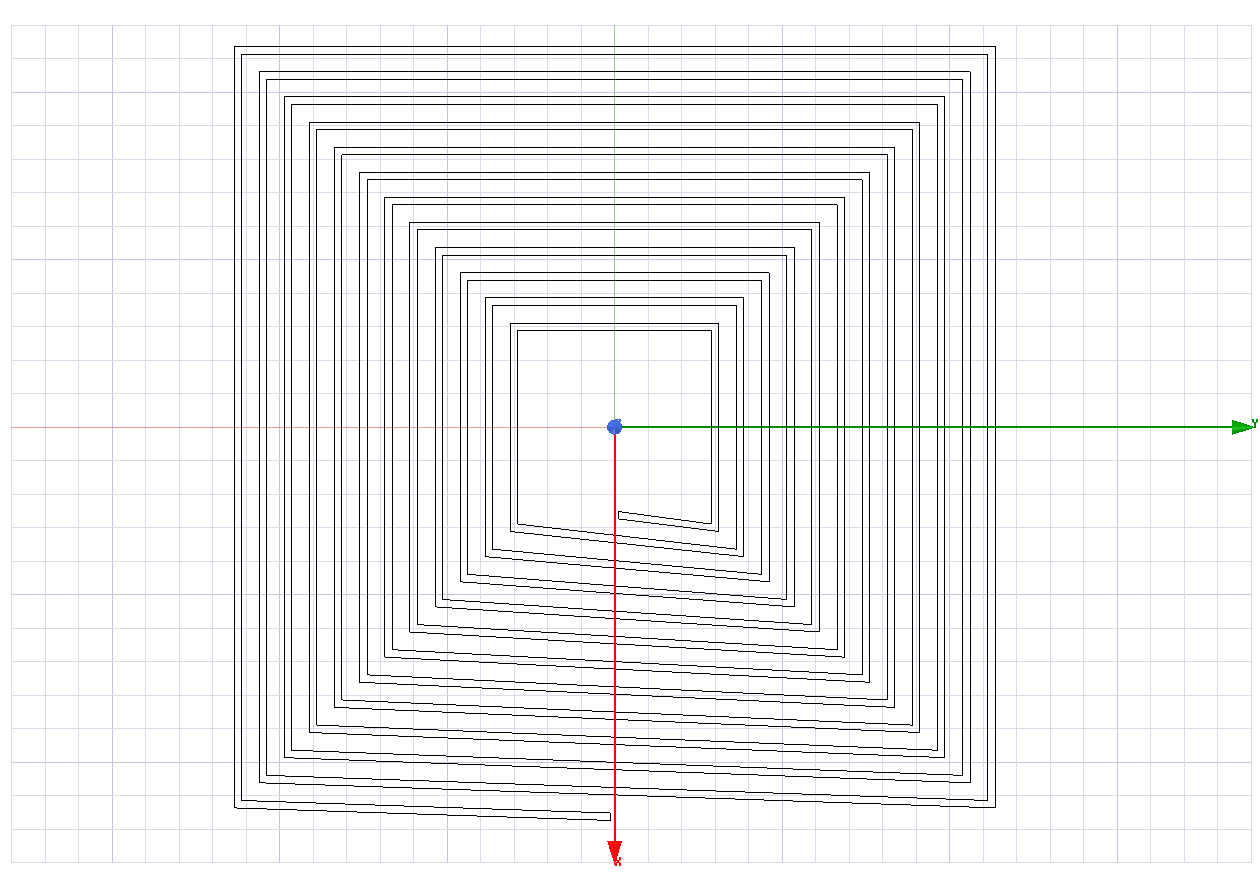
\includegraphics[width=0.8\linewidth]{./figures/example-curve.png}}\par
  \subcaptionbox{最终完成的几何模型\label{fig:example-overall}}
    {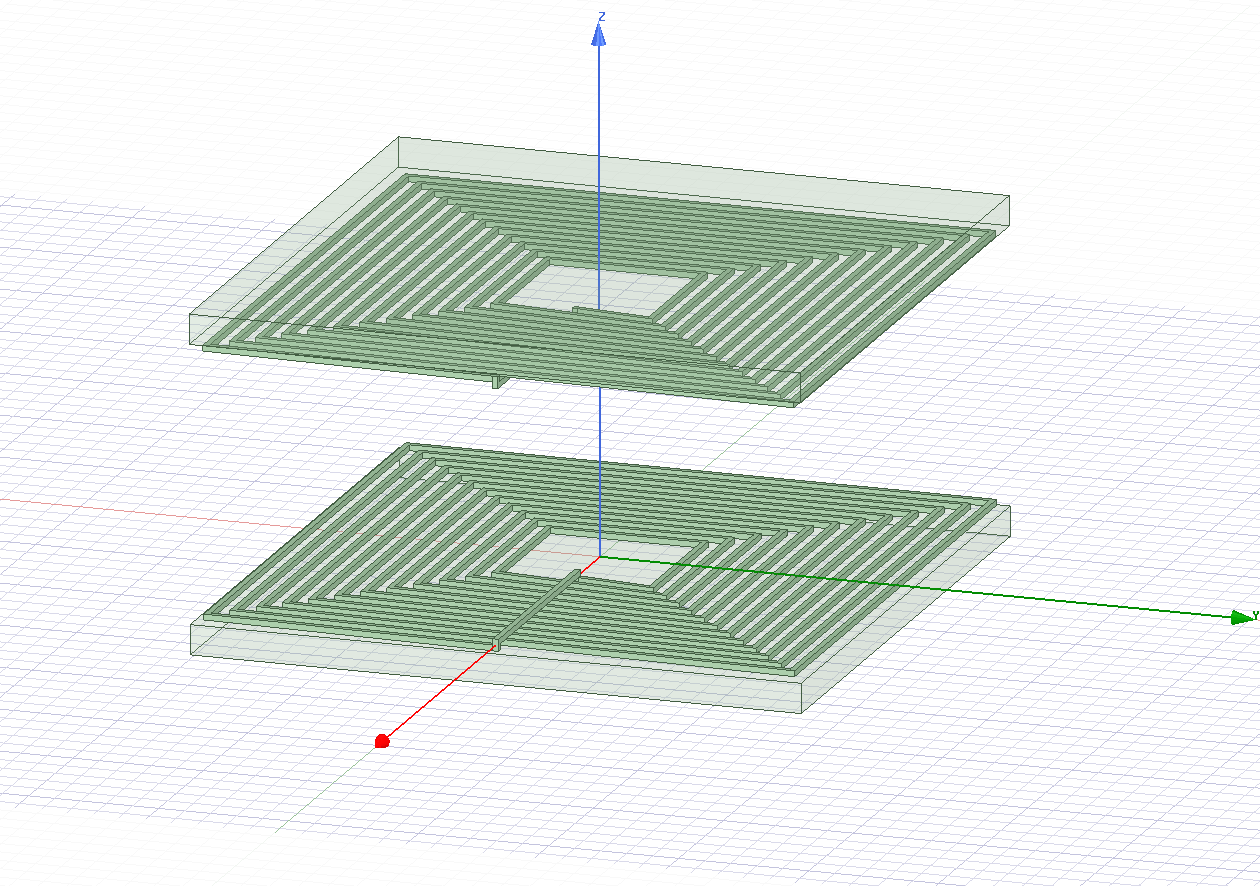
\includegraphics[width=0.8\linewidth]{./figures/example-overall.png}}
  \caption[几何模型的搭建]{使用Ansys Maxwell 3D对磁谐振部件的几何结构进行建模。}
\end{figure}
有限元分析中最基础的一步就是搭建几何模型。为了与自动化设计系统结合,需要尽可能地对所有几何结构进行参数化。
图\cref{fig:example-model,fig:example-overall}给出了已经搭建好的几何模型的逻辑结构和直观样子。
虽然其中磁屏蔽层和空气的建模乏善可陈,但线圈的几何结构建模需要略作讨论。

首先,本文采用截面积相等的正方形截面替代圆形截面对线圈进行建模,以大大降低计算量。
其次,本文利用参数曲线的方法来对方形线圈的复杂螺旋结构进行建模
(参数曲线如\cref{fig:example-curve}所示;由于其具体表达式异常复杂,将在\cref{sec:tricks}中给出)。
最后,本文用简单放样和布尔运算将螺旋结构的首位相连,得到完整的线圈模型。

\subsection{设置磁参数}
在有了几何模型之后,需要指定材料、边界和激励。
本文将所采用PC95铁氧体材料的磁导率导入Ansys Maxwell中,并分别设定磁屏蔽层的材料为PC95、线圈的材料为铜。
由于开放空间中不涉及对称性问题,故无需指定边界条件。
最后,添加两个绕组(Winding)——发射和接收线圈——及其终端(Terminal)。
\cref{fig:example-proj}

\subsection{设置仿真参数}
为了得到所需的信息(电阻和电感),选取交变电流(EddyCurrent)分析方法,添加阻抗矩阵仿真参数,
设置求解步骤(此处需要使用系统工作频率\SI{85}{\kilo\hertz})。

\section{约束条件与设计目标}
% TODO
\section{运行结果}
% TODO
\end{document}
